
\begin{enumerate}
\item 
\question{If I have an RC circuit with a resistor of $10\myohm$ and a capacitor of $2\myf$, what is the RC time constant of this circuit?}
\solution{$20$ seconds}
\explanation{The RC time constant is just the resistance (in ohms) multiplied by the capacitance (in farads).
Therefore, multiply $10\cdot 2 = 20$.
The time constant is $20$ seconds.
}
\item 
\question{In the previous question, how many seconds does it take to charge my capacitor to approximately 50\% of supply voltage?}
\solution{$14$ seconds}
\explanation{Figure~\ref{figTimeConstants} shows how many time constants it takes to charge a capacitor to a certain percentage of supply voltage.
Like most things in electronics, it won't be exact.
However, in the figure you can see that $0.7$ time constants will yield 50.3\% of the supply voltage.
Since the time constant was $20$ seconds, the amount of time to charge 50\% is $0.7\cdot 20 = 14$ seconds.
}
\item 
\question{If I have an RC circuit with a resistor of $30,000\myohm$ and a capacitor of $0.001\myf$, what is the RC time constant of this circuit?}
\solution{$30$ seconds}
\explanation{The RC time constant is just resistance (in ohms) multiplied by capacitance (in farads).
In this case, that yields $30,000 \cdot 0.001 = 30$ seconds.
}
\item 
\question{In the previous question, what percentage of the way is the capacitor's voltage charged after 60 seconds?}
\solution{86.5\%}
\explanation{Since the RC time constant is 30 seconds, 60 seconds would be two RC time constants.
Figure~\ref{figTimeConstants} shows that two time constants yields an 86.5\% voltage charge.}
\item 
\question{If I have an RC circuit with a resistor of $25\mykohm$ and a capacitor of $20\myuf$, what is the RC time constant of this circuit?}
\solution{$0.25$ seconds}
\explanation{This is just like the other time constant problems, except that we have to change units.
The units for the RC circuit are ohms and farads.
Since $1\mykohm = 1,000\myohm$, then $25\mykohm = 25,000\myohm$.
Likewise, since $1\myuf = 0.000001\myf$, then $20\myuf = 0.00002\myf$.

Now we just need to multiply them together.
$25,000 \cdot 0.00002 = 0.5$ seconds.
}
\item 
\question{Give a resistor and capacitor combination that will yield an RC time constant of 0.25 seconds.}
\solution{Any resistor/capacitor combination that, when multiplied together, yields $0.25$ will suffice.  A simple example would be to halve \emph{one} of the component values from the previous problem. For instance, I could keep the $25\mykohm$ resistor but change the capacitor to $10\myuf$.}
\item 
\question{Reconfigure the circuit in Figure~\ref{figSimpleTimerCircuit} to wait for 3 seconds.  Draw the whole circuit.}
\solution{There are an infinite number of ways to modify this solution to achieve your goal.  An example one is: \newline
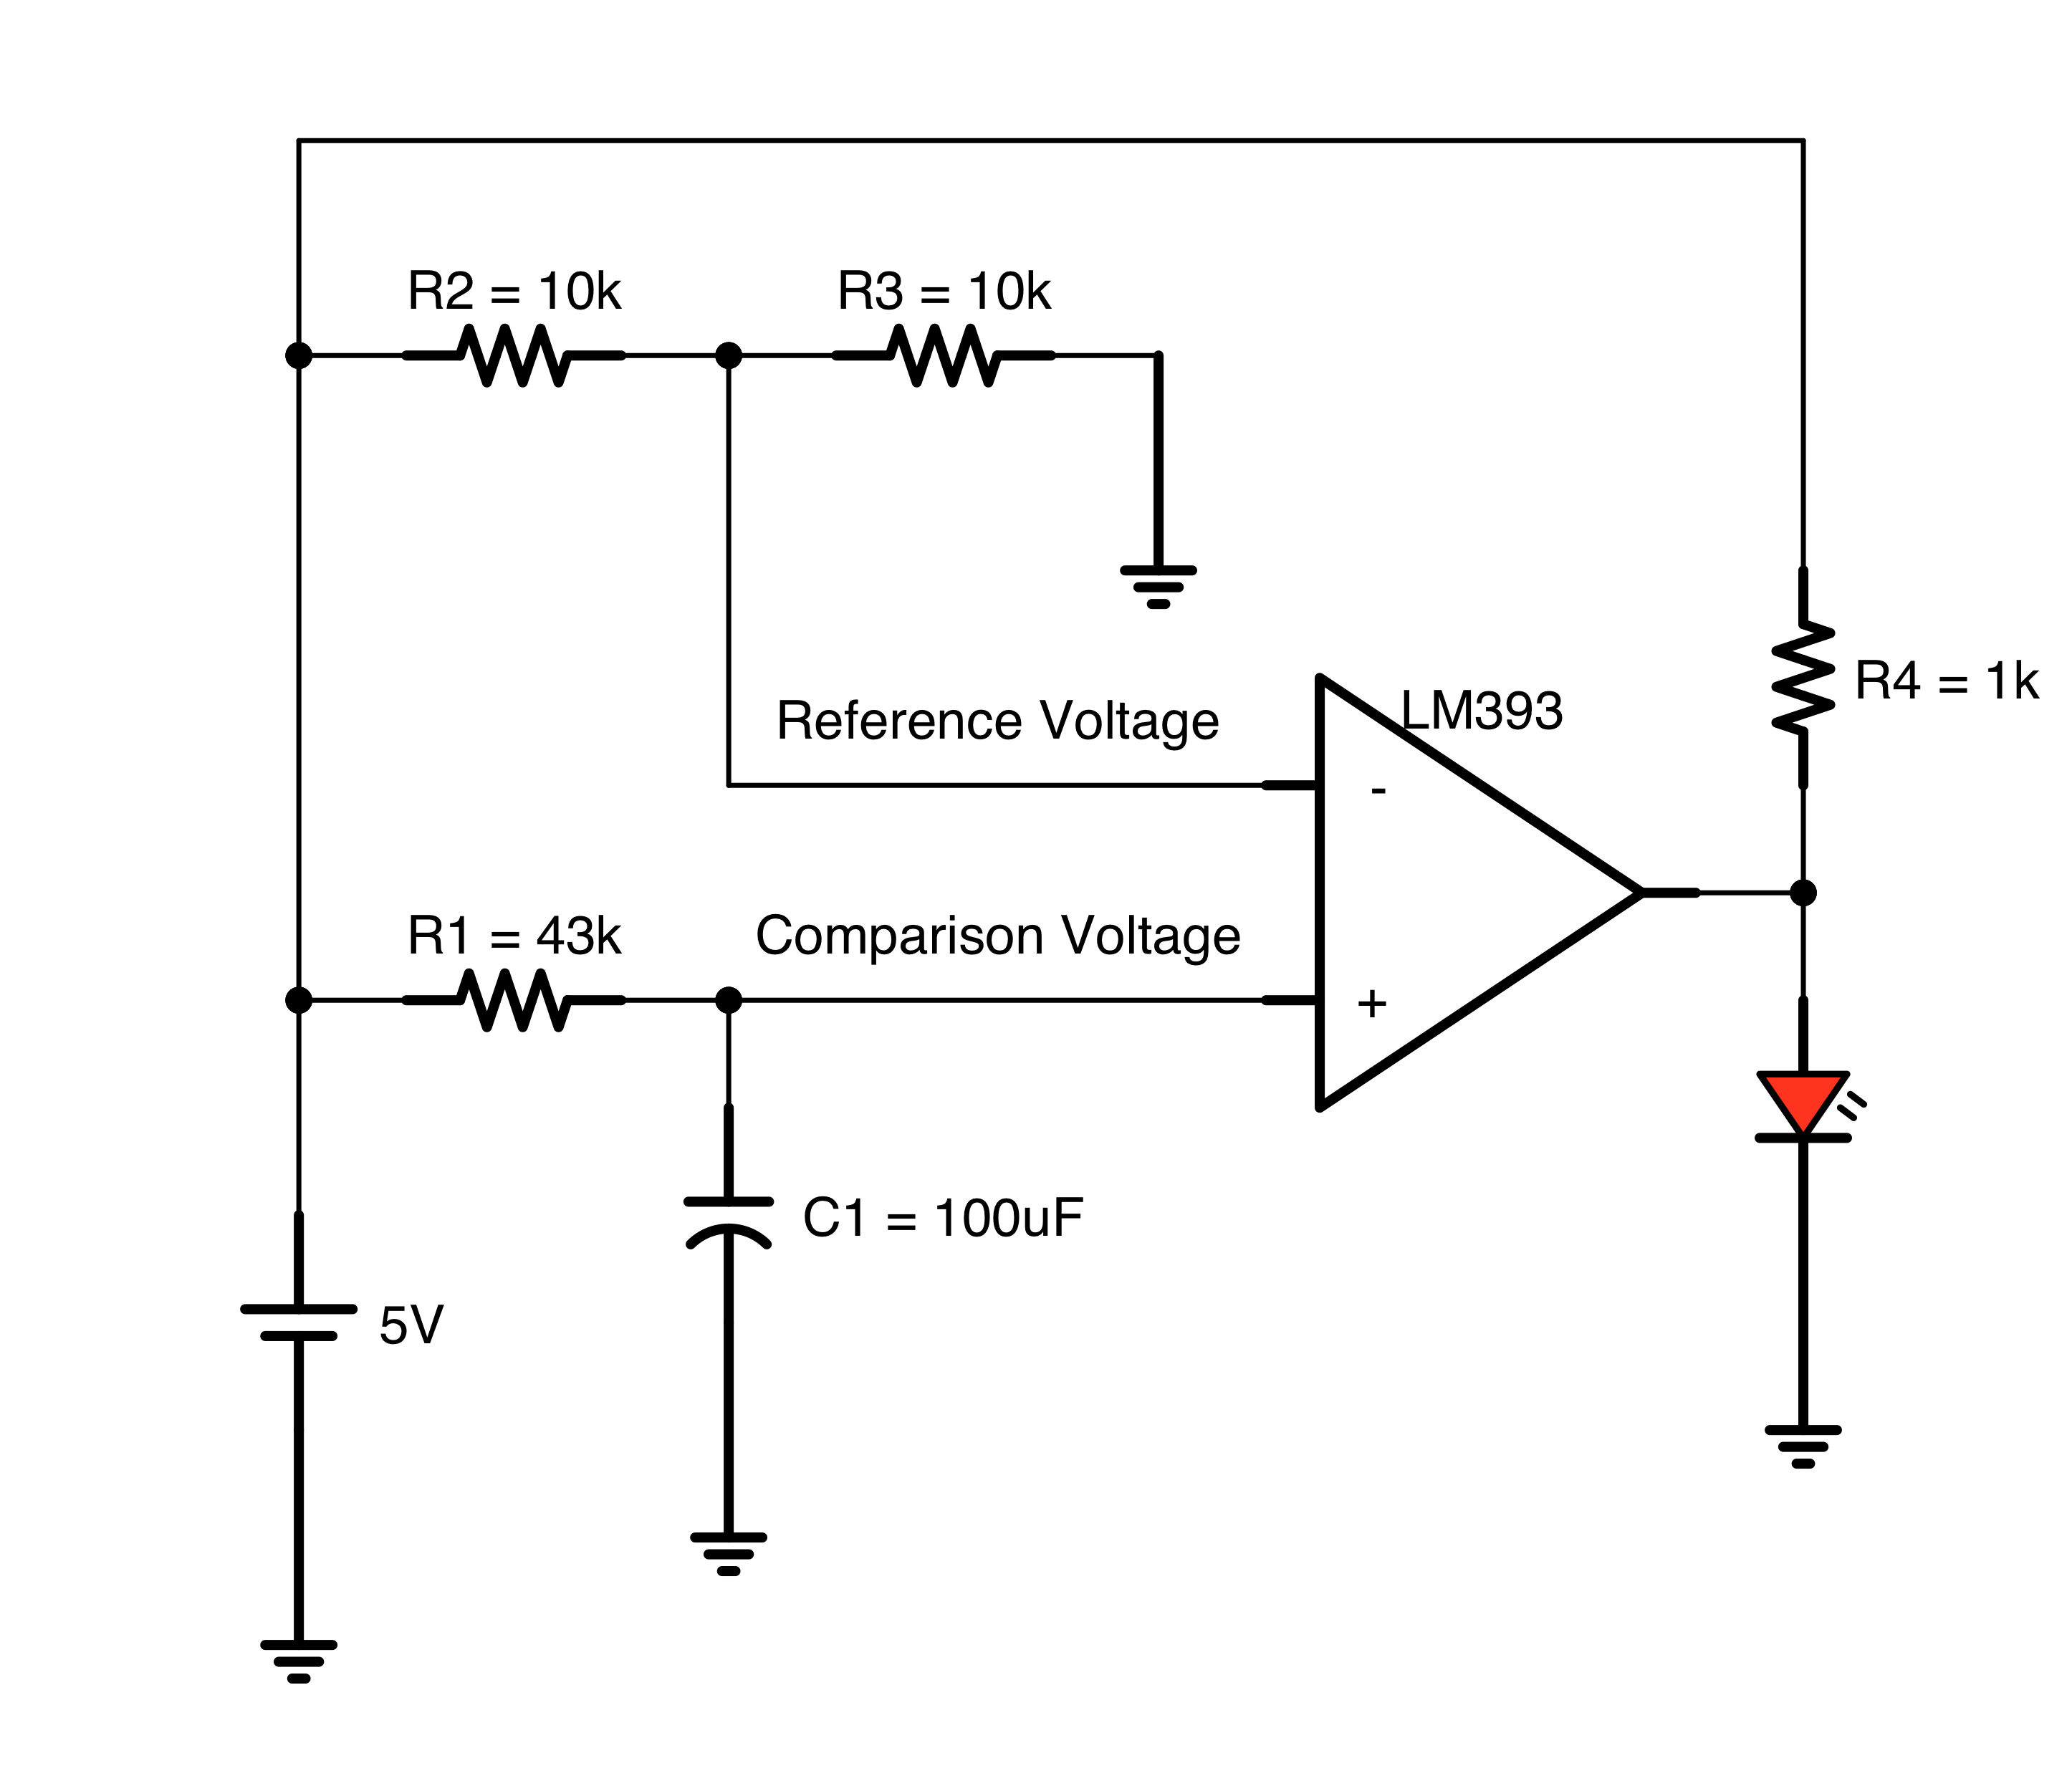
\includegraphics[width=0.7\columnwidth]{SolutionSimpleTimerCircuit}
}
\explanation{The way that the circuit works is by comparing the comparison voltage to the reference voltage.
Since the reference voltage is produced by a voltage divider, we can see that the output of the voltage divider will be 50\% of voltage, or $2.5\myvolt$.
Therefore, when the comparison voltage rises above $2.5\myvolt$, the comparator will fire.
According to Figure~\ref{figTimeConstants}, the capacitor will be 50\% full (thus making the comparison voltage over $2.5\myvolt$ after $0.7$ time constants.

Therefore, since we are wanting a waiting period of $3\mysec$, we can solve for the time constant $C$ like this:
\begin{align*}
3\mysec &= 0.7 \cdot C \\
\frac{3\mysec}{0.7} &= C \\
4.3\mysec &= C
\end{align*}

Therefore, we need a time constant of $4.3\mysec$.
The time constant is found by multiplying the resistance times the capacitance.
Therefore, R1 and C1 can be \emph{any} values that multiply to be approximately $4.3$.
In the example above, we merely changed the resistor to be $43,000\myohm$ ($43\mykohm$), because $43,000 \cdot 0.0001 = 4.3$.
}
\item 
\question{Redraw the previous circuit, and circle each basic resistor circuit pattern and label it.}
\solution{Using the circuit from the previous question, it should be labeled as follows: \newline
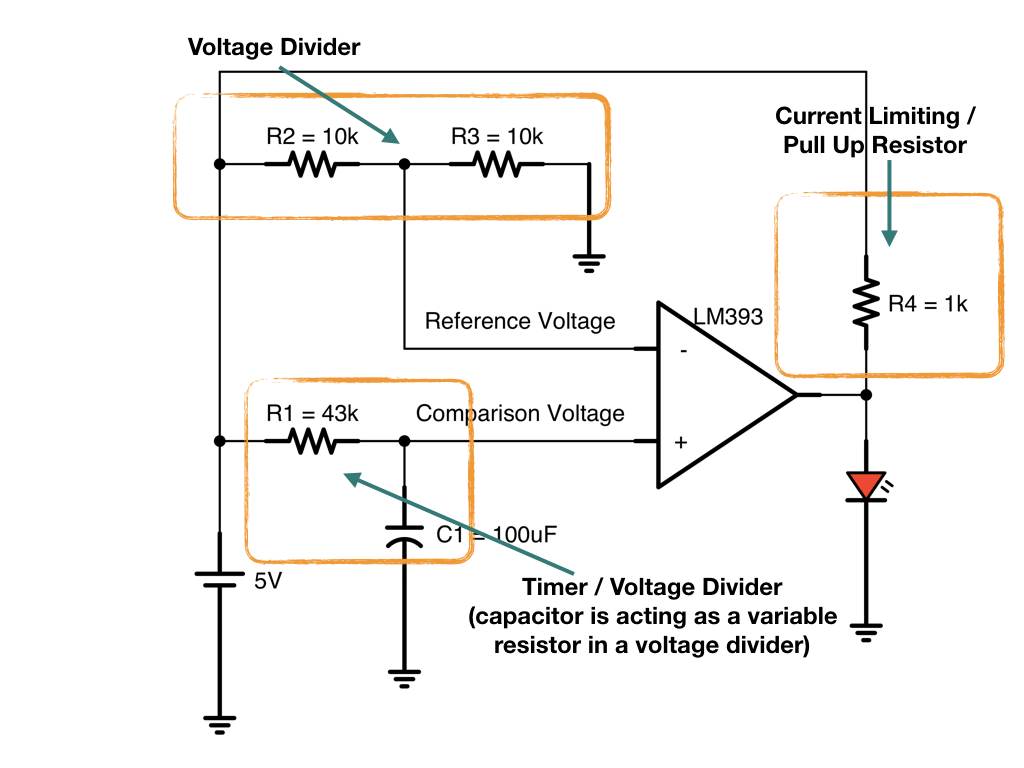
\includegraphics[width=0.8\columnwidth]{CapacitorTimerLabeled.png}
}
\explanation{
This circuit uses three resistor circuit patterns.
The reference voltage is set using a voltage divider circuit.
The timing circuit itself is a voltage divider as well, even though it includes a capacitor.
The capacitor acts as a sort of variable resistor, increasing the voltage across it as it fills.
Thus, the voltage coming out from between the resistor and the capacitor changes based on how full the capacitor is.
Finally, the resistor attached to the LED is a pull-up resistor.
Pull-up resistors also function as current-limiting resistors (however, simply labeling it as a pull-up resistor is sufficient).
}
\end{enumerate}
